\documentclass[12pt]{article}

\usepackage{amsmath}
\usepackage{graphicx}
\usepackage{subfigure}
\usepackage{float}
\usepackage{ulem}
\usepackage{bm}

\usepackage{anysize}

\marginsize{2cm}{2cm}{0.9cm}{1.8cm}
\usepackage[framed,numbered,autolinebreaks,useliterate]{mcode}
\usepackage{listings}
\lstset{language=Matlab}
\lstset{breaklines}
\lstset{extendedchars=false}

\title{Machine Learning/Pattern Recognition\\  \begin{Large} Homework \#2 \end{Large} }
\author{Jiyu Tian}
\date{}


\begin{document}

\maketitle
%%---------------------------------------------------------------
%% Problem 1
%%---------------------------------------------------------------
\section{Problem 2.12}
\large{\textbf{Solution}}: \\
(a) From normalization condition we have:\\
\begin{equation*}
1 = \sum_{i=1}^{c} P(w_i|\bm{x}) \leq \sum_{i=1}^{c} P(w_{max}|\bm{x}) = c\times P(w_{max}|\bm{x})
\end{equation*}
And therefore we must have:
\begin{equation*}
P(w_{max}|\bm{x})\leq \frac{1}{c}
\end{equation*}
(b) The probability of error is 1 minus the probability of being correct, that is:
\begin{equation*}
\begin{aligned}
P(error) &= 1 - P(correct)\\ &= 1-\int P(correct|\bm{x})P(\bm{x}) \text{ d}\bm{x}\\ & = 1-\int P(w_{max}|\bm{x})P(\bm{x}) \text{ d}\bm{x}
\end{aligned}
\end{equation*}
(c) With two results above we have:
\begin{equation*}
\begin{aligned}
P(error)&=1-\int P(w_{max}|\bm{x})P(\bm{x})\text{ d}\bm{x}\\ &\leq 1- \frac{1}{c}\int P(\bm{x})\text{ d}\bm{x}\\ &= 1-\frac{1}{c}
\end{aligned}
\end{equation*}
(d) Equality occurs if and only if all posteriors are equal:
\begin{equation*}
P(w_i|\bm{x})=P(w_j|\bm{x}) \text{ for all }i,j=1,...,c
\end{equation*}


\vfill
\clearpage
%%---------------------------------------------------------------
%% Problem 2
%%---------------------------------------------------------------
\section{Problem 3.1}
\large{\textbf{Solution}}: \\
(a) Figure 1 can be plotted with MATLAB:
\begin{figure}[H]
\centering
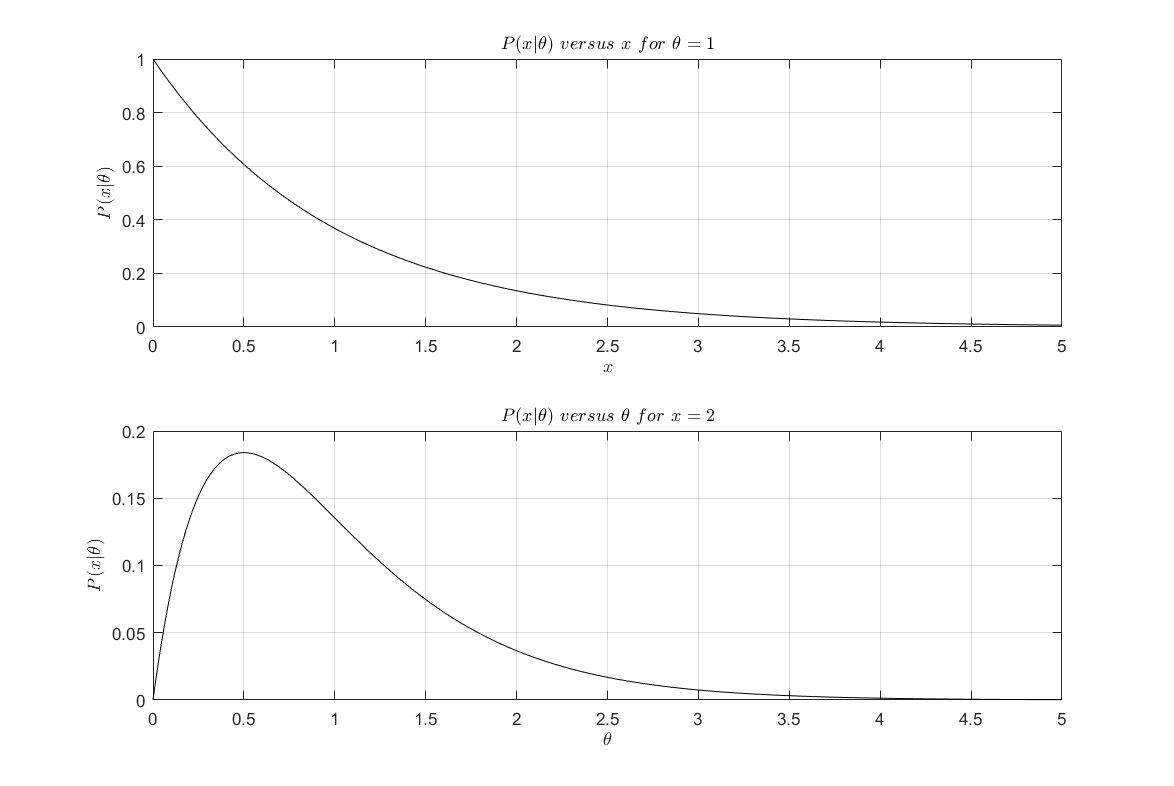
\includegraphics[width = 1\textwidth]{PR31.png}
\caption{\label{fig2}$P(x|\theta)\ versus\ x\ and\ \theta$}
\end{figure}
\noindent(b) \\
\begin{equation*}
\begin{aligned}
\hat{\theta} &=\arg\max_{\theta}\ P(D|\theta) = \arg\max_{\theta}\ \prod_{i=1}^{n} P(x_i|\theta) =\arg\max_{\theta}\ \prod_{i=1}^{n} \theta e^{-\theta x_i}\\ &=\arg\max_{\theta}\ \theta^n e^{-\theta \sum^{n}_{i=1}x_i} =\arg\max_{\theta}\ n\text{ln}\theta-\theta \sum^{n}_{i=1}x_i
\end{aligned}
\end{equation*}
Taking the derivative and equating to 0, we have:
\begin{equation*}
\begin{aligned}
\frac{n}{\hat{\theta}}-\sum^{n}_{i=1}x_i = 0
\end{aligned}
\end{equation*}
Then the maximum likelihood estimator $\hat{\theta}$ is given by
\begin{equation*}
\hat{\theta}=\frac{1}{\frac{1}{n}\sum^{n}_{i=1}x_i}.
\end{equation*}

\vfill
\clearpage
%%---------------------------------------------------------------
%% Problem 3
%%---------------------------------------------------------------
\section{Problem 3.2}
\large{\textbf{Solution}}: \\
(a) Here we introduce an indicator function $\bm{1}\{\cdot\}$ which equals to 1 for condition within and 0 otherwise. 
\begin{equation*}
\begin{aligned}
\hat{\theta} &=\arg\max_{\theta}\ P(D|\theta) = \arg\max_{\theta}\ \prod_{i=1}^{n} P(x_i|\theta) =\arg\max_{\theta}\ \prod_{i=1}^{n} \frac{1}{\theta}\ \bm{1}\{0\leq x_i\leq \theta\}\\ 
&=\arg\max_{\theta}\  \frac{1}{\theta^n} \prod_{i=1}^{n}\bm{1}\{0\leq x_i\leq \theta\}\\ 
&= \arg\max_{\theta}\  \frac{1}{\theta^n}\ \bm{1}\{0\leq\min_i x_i\}\ \bm{1}\{\max_i x_i\leq\theta\}
\end{aligned}
\end{equation*}
The function equals to zero for $\theta\leq \underset{i}{\max}\ x_i$ and decreases as $\theta$ increases for $\theta\geq \underset{i}{\max}\ x_i$.  Therefore, the likelihood function is maximized at $\hat{\theta} =  \underset{i}{\max}\ x_i$.
%%---------------------------------------------------------------
%% Problem 4
%%---------------------------------------------------------------
\section{Problem 3.3}
\large{\textbf{Solution}}: \\
(a) From statement we have $P\{z_{ik}=1|P(w_i)\}=P(w_i)$ and $P\{z_{ik}=0|P(w_i)\}=1-P(w_i)$, which can be combined as:
\begin{equation*}
\begin{aligned}
P(z_{ik}|P(w_i))=P(w_i)^{z_{ik}}(1-P(w_i))^{1-z_{ik}}
\end{aligned}
\end{equation*}
Then for the independent states, we have:
\begin{equation*}
\begin{aligned}
P(z_{i1},...,z_{ik}|P(w_i))=\prod^n_{k=1}P(z_{ik}|P(w_i))=\prod^n_{k=1}P(w_i)^{z_{ik}}(1-P(w_i))^{1-z_{ik}}
\end{aligned}
\end{equation*}
(b) With $\theta = P(w_i)$, the ML estimate for $P(w_i)$ can be expressed as:
\begin{equation*}
\begin{aligned}
\hat{\theta} &= \arg\max_{\theta}\ \prod^n_{k=1}\theta^{z_{ik}}(1-\theta)^{1-z_{ik}} =\arg\max_{\theta}\ \sum_{k=1}^{n} [z_{ik}\ln\theta+(1-z_{ik})\ln(1-\theta)]
\end{aligned}
\end{equation*}
Taking the derivative and equating to 0, we have:
\begin{equation*}
\begin{aligned}
\frac{1}{\hat{\theta}}\ \sum_{k=1}^{n} z_{ik} - \frac{1}{1-\hat{\theta}}\ \sum_{k=1}^{n} (1-z_{ik}) = 0\\
\end{aligned}
\end{equation*}
\begin{equation*}
\begin{aligned}
\hat{P}(w_i)=\hat{\theta} = \frac{1}{n}\sum_{k=1}^{n} z_{ik}
\end{aligned}
\end{equation*}
The ML estimate of prior probability is merely the number of this category divided by total number of samples.
\vfill
\clearpage
%%---------------------------------------------------------------
%% Problem 5
%%---------------------------------------------------------------
\section{Problem 3.4}
\large{\textbf{Solution}}: \\
\begin{equation*}
\begin{aligned}
\hat{\bm{\theta}} &= \arg\max_{\bm{\theta}} \ln P(\bm{D}|\bm{\theta}) =  \arg\max_{\bm{\theta}} \ln \prod^n_{k=1}\prod^d_{i=1}\theta_i^{x_{ki}}(1-\theta_i)^{1-x_{ki}}\\
&=\arg\max_{\bm{\theta}} \sum^n_{k=1}\sum^d_{i=1}x_{ki}\ln\theta_i + (1-x_{ki})\ln(1-\theta_i)
\end{aligned}
\end{equation*}
Taking the partial derivative with respect to $\theta_i$ and equating to 0, we have:
\begin{equation*}
\begin{aligned}
\frac{1}{\hat{\theta_i}}\sum_{k=1}^n x_{ki} - \frac{1}{1-\theta_i} \sum_{k=1}^n (1-x_{ki}) =0
\end{aligned}
\end{equation*}

\begin{equation*}
\begin{aligned}
\hat{\theta_i} = \frac{1}{n} \sum_{k=1}^n x_{ki}
\end{aligned}
\end{equation*}
Therefore the ML estimate for $\bm{\theta}$ is 
\begin{equation*}
\begin{aligned}
\hat{\bm{\theta}} = \frac{1}{n} \sum_{k=1}^n x_{k}
\end{aligned}
\end{equation*}

%%---------------------------------------------------------------
%% Problem 6
%%---------------------------------------------------------------
\section{Problem 3.17}
\large{\textbf{Solution}}: \\
(a) For n $i.i.d$ samples $D=\{\bm{x}_1,...,\bm{x}_n\}$, we have:

\begin{equation*}
\begin{aligned}
P(D|\bm{\theta})&=P(\bm{x_1},...,\bm{x_n}|\bm{\theta}) = \prod_{k=1}^n P(x_k|\bm{\theta})\\ &= \prod_{k=1}^n \prod^d_{i=1} \theta_i^{x_{ki}}(1-\theta_i)^{1-x_{ki}} \\ &= \prod^d_{i=1} \theta_i^{\sum_{k=1}^n x_{ki}}(1-\theta_i)^{\sum_{k=1}^n (1-x_{ki})}\\ &= \prod^d_{i=1} \theta_i^{s_i}(1-\theta_i)^{n-s_i}
\end{aligned}
\end{equation*}
\noindent(b) With assumption that $\bm{\theta}$ is uniformly distributed, we have $P(\bm{\theta})=1$ for $0\leq \theta_i \leq1,\ i=1,...,d$. From Bayes' theorem we have:
\begin{equation*}
\begin{aligned}
P(\bm{\theta}|D)&=\frac{P(D|\bm{\theta})P(\bm{\theta})}{P(D)} =\frac{P(D|\bm{\theta})P(\bm{\theta})}{\int P(D|\bm{\theta})P(\bm{\theta})\text{ d}\bm{\theta}}= \frac{P(D|\bm{\theta})}{\int P(D|\bm{\theta})\text{ d}\bm{\theta}}\\
&= \frac{\prod^d_{i=1} \theta_i^{s_i}(1-\theta_i)^{n-s_i}}{\int \prod^d_{i=1} \theta_i^{s_i}(1-\theta_i)^{n-s_i}\text{ d}\bm{\theta}}\\
&=\frac{\prod^d_{i=1} \theta_i^{s_i}(1-\theta_i)^{n-s_i}}{\int_0^1 ... \int_0^1 \prod^d_{i=1} \theta_i^{s_i}(1-\theta_i)^{n-s_i}\text{ d}\theta_1...\text{d}\theta_d}\\
&=\prod_{i=1}^{d} \frac{\theta_i^{s_i}(1-\theta_i)^{n-s_i}}{\int_0^1 \theta_i^{s_i}(1-\theta_i)^{n-s_i}\text{ d}\theta_i}\\
&=\prod_{i=1}^{d} \frac{\theta_i^{s_i}(1-\theta_i)^{n-s_i}}{\frac{s_i!(n-s_i)!}{(n+1)!}}\\
&=\prod_{i=1}^{d} \frac{(n+1)!}{s_i!(n-s_i)!}\theta_i^{s_i}(1-\theta_i)^{n-s_i}\\
\end{aligned}
\end{equation*}
(c) Given $d=1,\ n=1$, we have: 
\begin{equation*}
\begin{aligned}
P(\theta|D)= \frac{2!}{s_1!(1-s_1)!}\theta^{s_1}(1-\theta)^{1-s_1}\\
\end{aligned}
\end{equation*}
Note that $s_1$ has two values 0 and 1, and the density for each of them:
\begin{equation*}
\begin{aligned}
&s_1 = 0\ :\ P(\theta|D)= 2(1-\theta)\\
&s_1 = 1\ :\ P(\theta|D)= 2\theta\\
\end{aligned}
\end{equation*}
The densities can be plotted with MATLAB as Figure 2.
\begin{figure}[H]
\centering
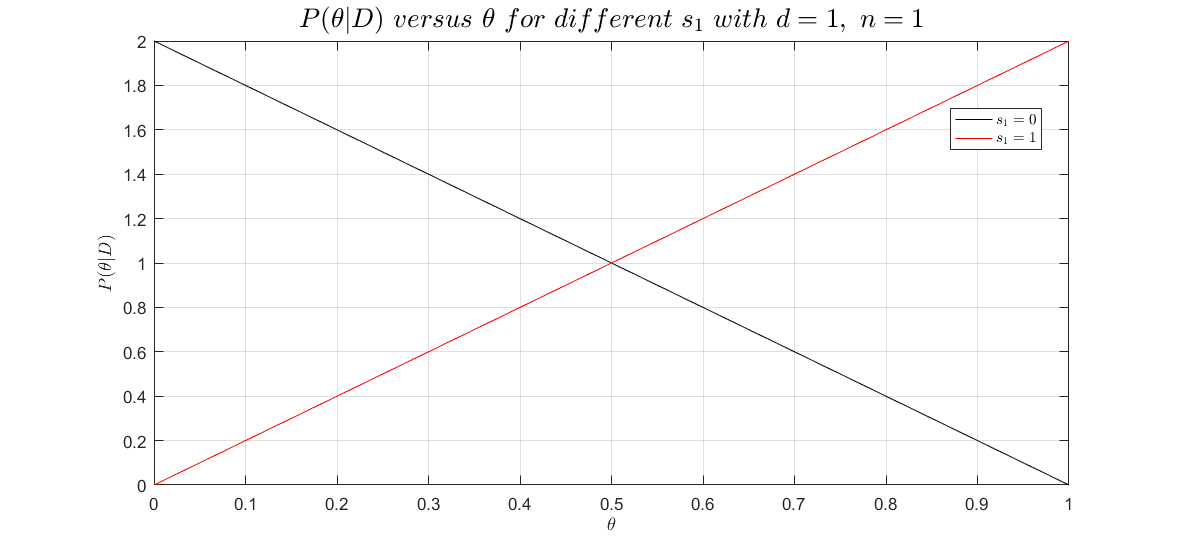
\includegraphics[width = 1\textwidth]{pb317.png}
\caption{\label{fig3}$P(x|\theta)\ versus\ x\ and\ \theta$}
\end{figure}
%------------------------------------------------------------------------
\noindent(d) Since in Bernoulli case $x_i$ can be either 0 or 1, we have:
\begin{equation*}
\begin{aligned}
P(\bm{x}|D) &= \int P(\bm{x}|\bm{\theta}) P(\bm{\theta}|D)\text{ d}\bm{\theta}\\ 
&=\int \prod_{i=1}^d\theta_i^{x_i}(1-\theta_i)^{1-x_i}\prod_{i=1}^{d} \frac{(n+1)!}{s_i!(n-s_i)!}\theta_i^{s_i}(1-\theta_i)^{n-s_i} \text{ d}\bm{\theta}\\
&=\prod_{i=1}^d  \frac{(n+1)!}{s_i!(n-s_i)!} \int \prod_{i=1}^d\theta_i^{x_i}(1-\theta_i)^{1-x_i} \theta_i^{s_i}(1-\theta_i)^{n-s_i} \text{ d}\bm{\theta}\\
&=\prod_{i=1}^d  \frac{(n+1)!}{s_i!(n-s_i)!} \prod_{i=1}^d \int \theta_i^{x_i+s_i}(1-\theta_i)^{n+1-x_i-s_i} \\
&=\prod_{i=1}^d  \frac{(n+1)!}{s_i!(n-s_i)!} \prod_{i=1}^d  \frac{(x_i+s_i)!(n+1-x_i-s_i)!}{(n+2)!} \\
&=\prod_{i=1}^d  \frac{(n+1)!(x_i+s_i)!(n+1-x_i-s_i)!}{s_i!(n-s_i)!(n+2)!} \\
&=\prod_{i=1}^d  \frac{(x_i+s_i)!(n+1-x_i-s_i)!}{s_i!(n-s_i)!(n+2)} \ \ \ \ \text{($x_i$ can be 0 or 1)}\\
&=\prod_{i=1}^d  (\frac{(s_i+1)!(n-s_i)!}{s_i!(n-s_i)!(n+2)})^{x_i} (\frac{s_i!(n+1-s_i)!}{s_i!(n-s_i)!(n+2)})^{1-x_i} \\
&=\prod_{i=1}^d  (\frac{s_i+1}{n+2})^{x_i} (\frac{n+1-s_i}{n+2})^{1-x_i} \\
&=\prod_{i=1}^d  (\frac{s_i+1}{n+2})^{x_i} (1-\frac{s_i+1}{n+2})^{1-x_i}
\end{aligned}
\end{equation*}





%-----------------------------------------------------------------------
\noindent(e) Comparing the following two equations:
\begin{equation*}
\begin{aligned}
P(\bm{x}|D) = \prod_{i=1}^d  (\frac{s_i+1}{n+2})^{x_i} (1-\frac{s_i+1}{n+2})^{1-x_i}
\end{aligned}
\end{equation*}
\begin{equation*}
\begin{aligned}
P(\bm{x}|\bm{\theta}) = \prod_{i=1}^d\theta_i^{x_i}(1-\theta_i)^{1-x_i}
\end{aligned}
\end{equation*}
we have the effective Bayesian estimate for $\bm{\theta}$:
\begin{equation*}
\begin{aligned}
\hat{\theta_i} = \frac{s_i+1}{n+2}
\end{aligned}
\end{equation*}


\end{document}


